\documentclass[11pt, oneside]{article} 
\usepackage{geometry}
\geometry{letterpaper} 
\usepackage{graphicx}
	
\usepackage{amssymb}
\usepackage{amsmath}
\usepackage{parskip}
\usepackage{color}
\usepackage{hyperref}

\graphicspath{{/Users/telliott/Dropbox/Github-Math/geoproof/figures/}{/Users/telliott/Dropbox/Github-Math/figures/}}
% \begin{center} \includegraphics [scale=0.4] {gauss3.png} \end{center}


\title{Ptolemy's theorem}
\date{}

\begin{document}
\maketitle
\Large

%[my-super-duper-separator]

\label{sec:Ptolemy}

Ptolemy was a Greek astronomer and geographer who probably lived at Alexandria in the 2nd century AD (died c. 168 AD).  That is nearly 500 years after Euclid.  Ptolemy was a popular name for Egyptian pharaohs in earlier centuries.

Our Ptolemy is known for many works including his book the \emph{Almagest}, and important to us, for a theorem in plane geometry concerning cyclic quadrilaterals.  These are 4-sided polygons all of whose vertices lie on a circle.  Recall that any triangle lies on a circle, so this is a restriction on the fourth vertex of the polygon.

A cyclic quadrilateral is a four-sided polygon whose vertices all lie in a circle.  Consider $ABCD$.  
\begin{center} 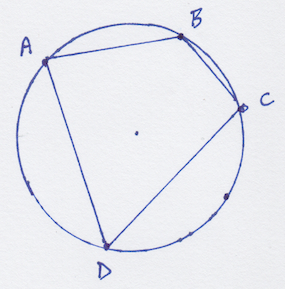
\includegraphics [scale=0.5] {O1.png} \end{center}

In this figure $\angle A$ and $\angle C$ are supplementary. The reason is that together, their arcs sweep out the entire circle.  The sum of all four peripheral angles is
\[ \angle A + \angle B + \angle C + \angle D = 360 \]

Of course we knew that, it is true for any four-sided polygon.

$\square$

Draw the diagonals $AC$ and $BD$.
\begin{center} \includegraphics [scale=0.5] {pt1.png} \end{center}

Ptolemy's theorem says that for a cyclic quadrilateral, the product of opposing sides, summed, is equal to the product of the diagonals:
\[ AB \cdot CD + BC \cdot AD = AC \cdot BD \]

\emph{Proof}.

I found a great proof without words here:

\url{https://www.cut-the-knot.org/proofs/PtolemyTheoremPWW.shtml}

We'll actually use some words in an attempt to see how one might have developed this proof.  We have switched to use single letters for the sides, and the angles are labeled with colored dots.  Equal angles come from the inscribed angle theorem.
\begin{center} \includegraphics [scale=0.4] {pt23.png} \end{center}

Now, the great idea is to construct a parallelogram.  We begin by cutting the figure in half along one of the diagonals, say $n$.  This makes two pieces from the other diagonal $m$, which we will ignore for the moment.
\begin{center} \includegraphics [scale=0.4] {pt24.png} \end{center}

Next, pick any two sides and align them horizontally.  
\begin{center} \includegraphics [scale=0.4] {pt25.png} \end{center}

At this point, we need to scale the figures to make a parallelogram.  Algebraically, we do this by multiplying.  Each of the three sides on the left is scaled by $d$, and each of three on the right by $a$.  
\begin{center} \includegraphics [scale=0.4] {pt26.png} \end{center}

We can also fill in the angles by referring back to the original diagram.  We have a parallelogram because the two short sides are equal and also parallel. 
\begin{center} \includegraphics [scale=0.4] {pt23.png} \end{center}
The angles in the new part of the parallelogram are determined by using the alternate interior angles theorem. Draw a central red line to help with placing the angles.

At this point, we realize that we have a matching triangle in the original figure.  It is the one with sides $a$, $d$ and $m$.  The red and green dotted angles are switched with respect to the central angle composed of red and magenta (the large triangle is a reflected version), but that's no problem.

It just needs to be scaled by $n$ to fit.
\begin{center} \includegraphics [scale=0.4] {pt27.png} \end{center}

As opposing sides in a parallelogram, the top and bottom must be equal in length.  Therefore
\[ mn = ac + bd \]

$\square$

\begin{center} \includegraphics [scale=0.5] {pt1.png} \end{center}

\subsection*{corollaries}

Here are just a few of the results that follow from this remarkable theorem.

\textbf{equilateral triangle}

\begin{center} \includegraphics [scale=0.4] {Ptolemy4.png} \end{center}

Inscribe an equilateral triangle in a circle and pick any point on the circle.

\[ qs = ps + rs \]
\[ q = p + r \]

\textbf{Pythagorean theorem}

Let the quadrilateral be a rectangle.  The the sum of squares of opposing sides is
\[ a^2 + b^2 \]

Triangles made by opposing diagonals are congruent, so the diagonals are equal in length.  The diagonal is the hypotenuse, hence
\[ a^2 + b^2 = h^2 \]

\textbf{golden mean in the pentagon}

\begin{center} \includegraphics [scale=0.3] {Ptolemy5.png} \end{center}

Take four vertices of the regular pentagon and draw two diagonals.  From the theorem, we have
\[ b \cdot b = a \cdot a + a \cdot b \]
\[ \frac{b^2}{a^2} = 1 + \frac{b}{a} \]

Rather than use the quadratic equation, rearrange and add $1/4$ to both sides to "complete the square":
\[ \frac{b^2}{a^2} - \frac{b}{a} + \frac{1}{2^2} = 1 + \frac{1}{2^2} \]

So
\[ (\frac{b}{a} - \frac{1}{2})^2  = \frac{5}{4} \]
\[ \frac{b}{a} - \frac{1}{2}  = \pm \ \frac{\sqrt{5}}{2} \]
\[ \frac{b}{a}  = \frac{1 \pm \sqrt{5}}{2} \]

This ratio $b/a$ is known as $\phi$, the golden mean.

We'll see one more result when we get to trigonometry.  All of the sum of angles formulas easily follow from Ptolemy's theorem.

\end{document}